\section{Evaluation}

\subsection{Execution Time}

\begin{figure}
\centering
\includegraphics[width=0.8\textwidth]{buildmodel}
\caption{\footnotesize Time to build the model, i.e. to generate association
rules, for the two algorithms with different minimum supports. }
\label{Fig:buildmodel}
\end{figure}

\begin{figure}
\centering
\includegraphics[width=0.8\textwidth]{TestingTime1}
\caption{\footnotesize Time to run the model over the test data, for algorithm
1 with different minimum supports and K values. }
\label{Fig:TestTime1}
\end{figure}

\begin{figure}
\centering
\includegraphics[width=0.8\textwidth]{TestingTime2}
\caption{\footnotesize Time to run the model over the test data, for algorithm
2 with different minimum supports and K values. }
\label{Fig:TestTime2}
\end{figure}

\subsection{Quality}
\subsubsection{Accuracy}

\begin{figure}
\centering
\includegraphics[width=0.8\textwidth]{Accuracy}
\caption{\footnotesize The accuracy for the two algorithms with different
parameters. }
\label{Fig:Accuracy}
\end{figure}

\subsubsection{F-measure}
\begin{figure}
        \centering
        \begin{subfigure}[b]{0.4\textwidth}
         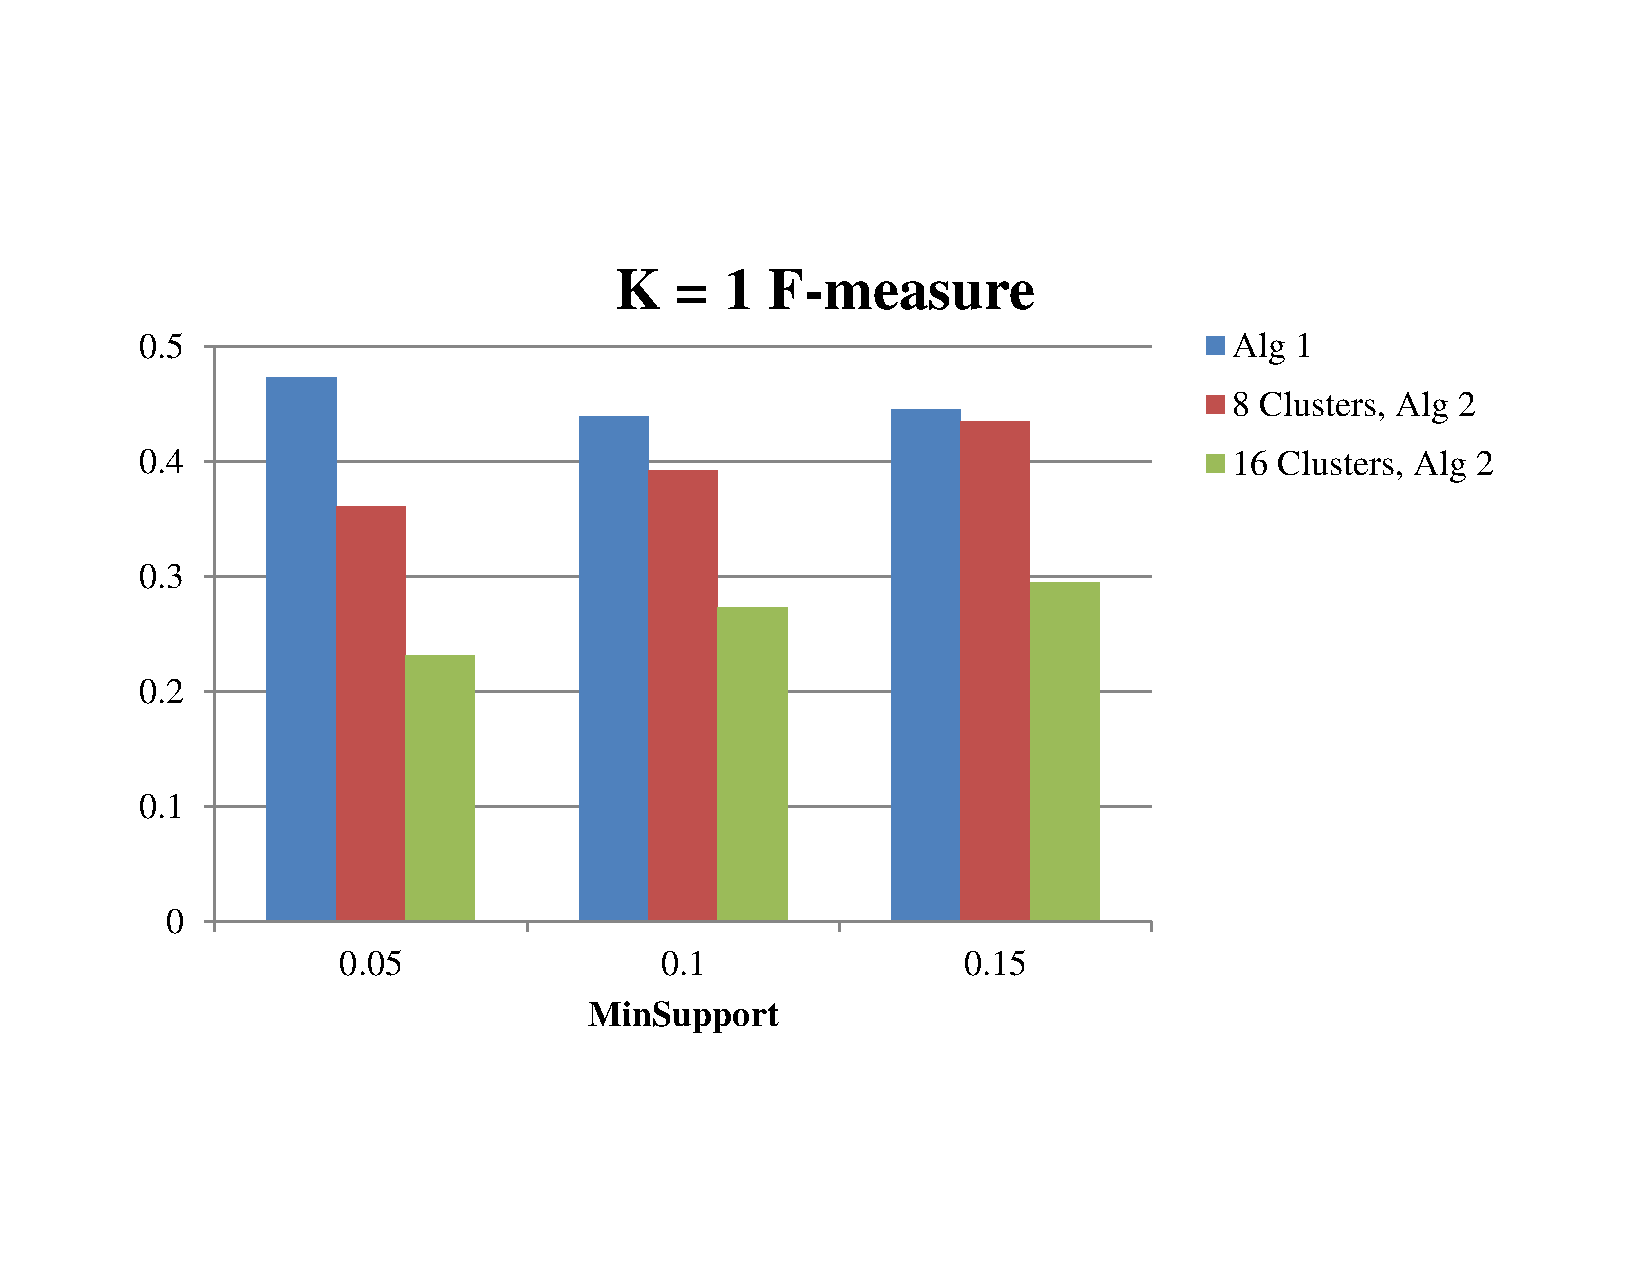
\includegraphics[width=\textwidth]{F-measure1}
         \caption{K = 1}
         \label{Fig:F-measure1}
        \end{subfigure}
        \begin{subfigure}[b]{0.4\textwidth}
         \includegraphics[width=\textwidth]{F-measure2}
         \caption{K = 2}
         \label{Fig:F-measure2}
        \end{subfigure}
        \begin{subfigure}[b]{0.4\textwidth}
         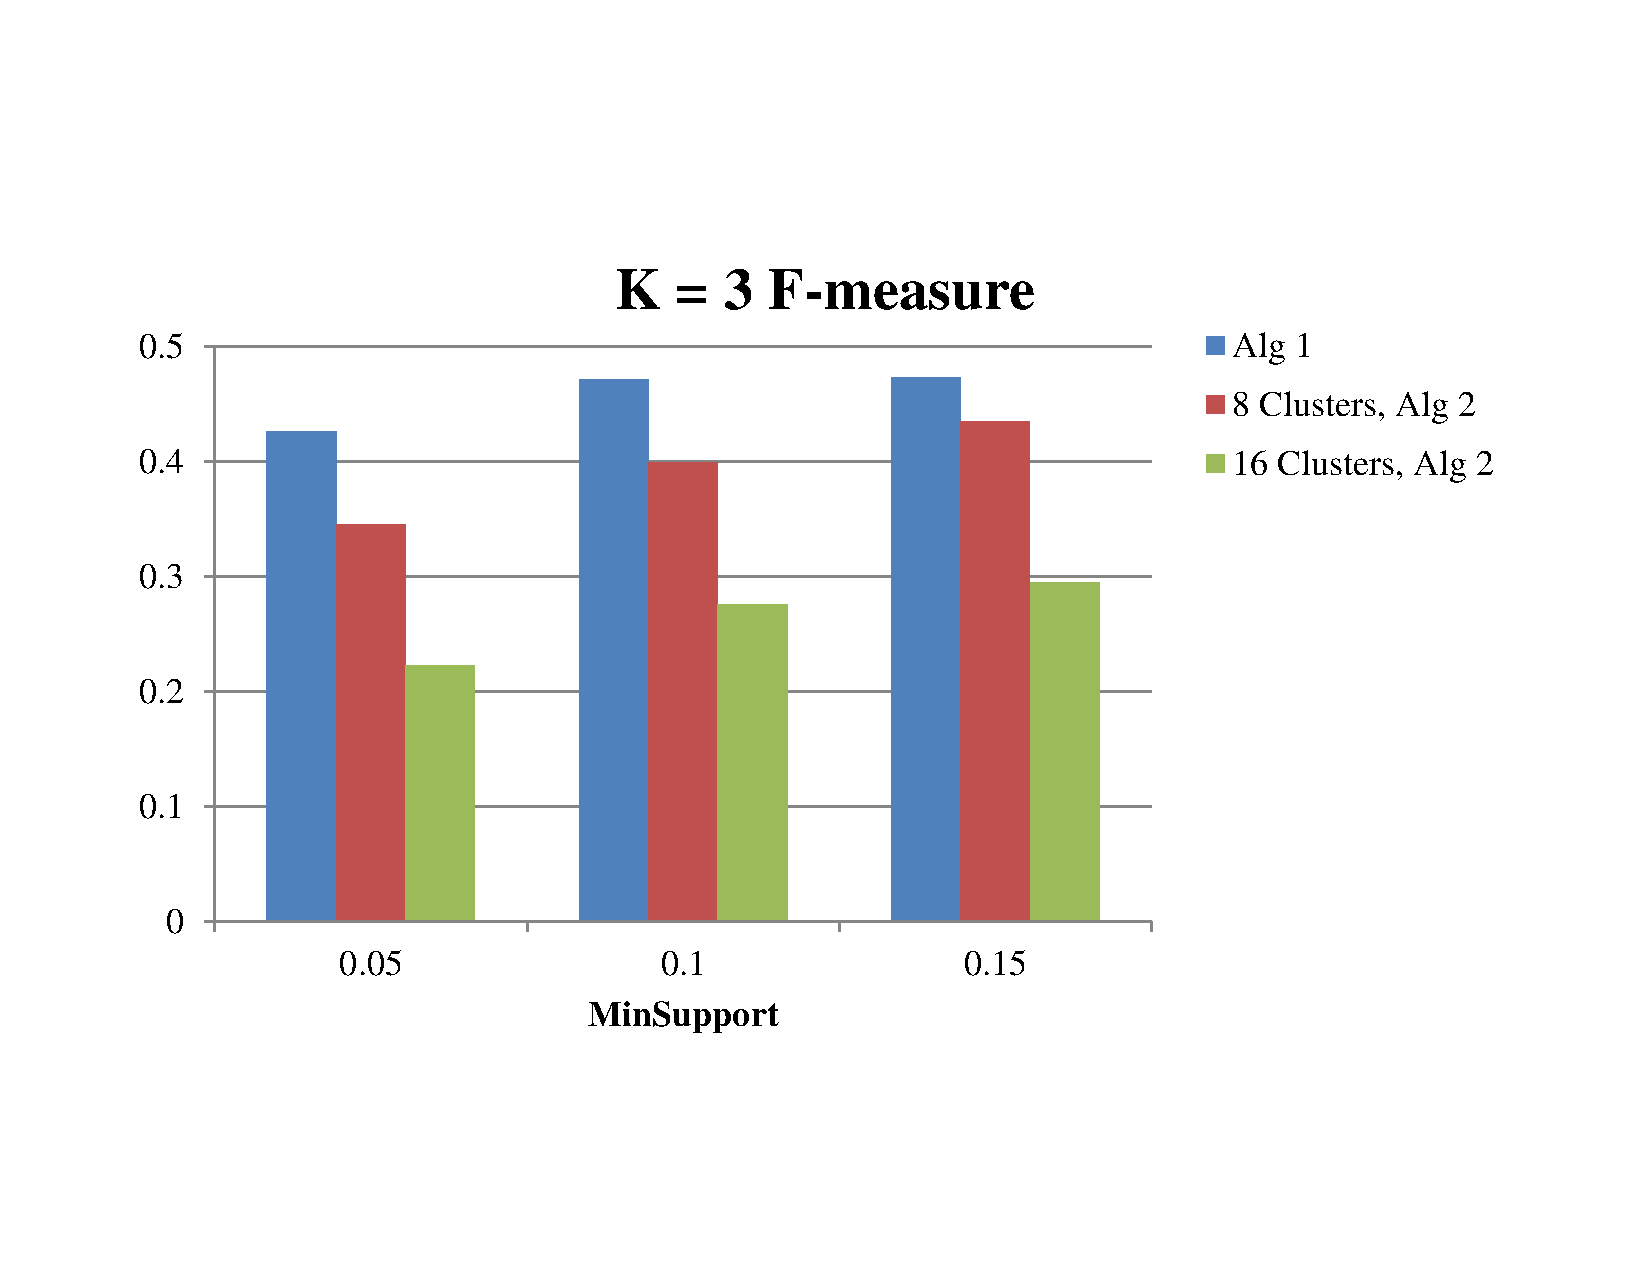
\includegraphics[width=\textwidth]{F-measure3}
         \caption{K = 3}
         \label{Fig:F-measure3}
        \end{subfigure}
        \begin{subfigure}[b]{0.4\textwidth}
         \includegraphics[width=\textwidth]{F-measure4}
         \caption{K = 4}
         \label{Fig:F-measure4}
        \end{subfigure}
        \begin{subfigure}[b]{0.4\textwidth}
         \includegraphics[width=\textwidth]{F-measure5}
         \caption{K = 5}
         \label{Fig:F-measure5}
        \end{subfigure}
        \caption{F-measures for two algorithms with different parameters.}
        \label{Fig:F-measure}
\end{figure}

\subsubsection{Skew}
